\documentclass[11pt]{article}
\usepackage{tikz}
%\usepackage{amsfonts}
\usetikzlibrary{automata, arrows}

\title{Homework \#2}
\author{Kyle White}
\date{March 5, 2017}

\begin{document}
\maketitle

\noindent1.3)
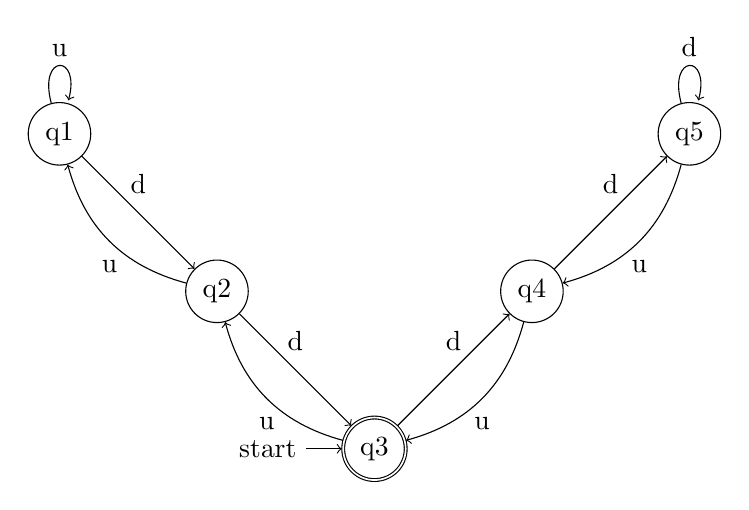
\begin{tikzpicture}

\tikzset{vertex/.style = {shape=circle,draw,minimum size=1em}}
\tikzset{edge/.style = {->,> = latex'}}
% vertices
\node[vertex] (1) at  (0,4) {q1};
\node[vertex] (2) at  (2,2) {q2};
\node[vertex, initial, accepting] (3) at  (4,0) {q3};
\node[vertex] (4) at (6,2) {q4};
\node[vertex] (5) at (8,4) {q5};
%edges

\path (1) edge[loop above] node {u} (1);
\draw [->] (1) -- (2) node [midway, label=above: d] {};
\draw [->] (2) -- (3) node [midway, label=above: d] {};
\draw [->] (3) -- (4) node [midway, label=above: d] {};
\draw [->] (4) -- (5) node [midway, label=above: d] {};
\draw [->] (2) edge[bend left] node [label=below: {u}] {} (1);
\draw [->] (3) edge[bend left] node [label=below: {u}] {} (2);
\draw [->] (4) edge[bend left] node [label=below: {u}] {} (3);
\draw [->] (5) edge[bend left] node [label=below: {u}] {} (4);
\path (5) edge[loop above] node {d} (5);

\end{tikzpicture}


\noindent1.4a)
\\
Accepts at least 3 a's

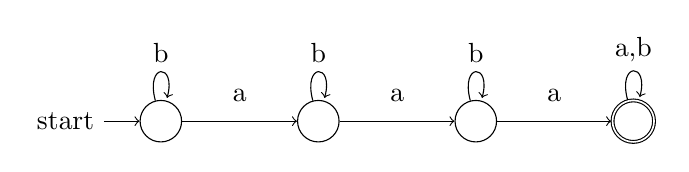
\begin{tikzpicture}

\tikzset{vertex/.style = {shape=circle,draw,minimum size=1.5em}}
\tikzset{edge/.style = {->,> = latex'}}
%verticies
\node[vertex, initial] (1) at  (0,0) {};
\node[vertex] (2) at  (2,0) {};
\node[vertex] (3) at  (4,0) {};
\node[vertex, accepting] (4) at  (6,0) {};
%edges
\draw [->] (1) -- (2) node [midway, label=above: a] {};
\draw [->] (2) -- (3) node [midway, label=above: a] {};
\draw [->] (3) -- (4) node [midway, label=above: a] {};
\path (1) edge[loop above] node {b} (1);
\path (2) edge[loop above] node {b} (2);
\path (3) edge[loop above] node {b} (3);
\path (4) edge[loop above] node {a,b} (4);

\end{tikzpicture}


\noindent Accepts at least 2 b's

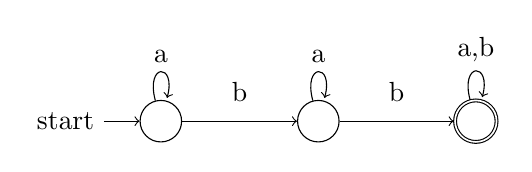
\begin{tikzpicture}

\tikzset{vertex/.style = {shape=circle,draw,minimum size=1.5em}}
\tikzset{edge/.style = {->,> = latex'}}
%verticies
\node[vertex, initial] (1) at  (0,0) {};
\node[vertex] (2) at  (2,0) {};
\node[vertex, accepting] (3) at  (4,0) {};
%edges
\draw [->] (1) -- (2) node [midway, label=above: b] {};
\draw [->] (2) -- (3) node [midway, label=above: b] {};
\path (1) edge[loop above] node {a} (1);
\path (2) edge[loop above] node {a} (2);
\path (3) edge[loop above] node {a,b} (3);

\end{tikzpicture}

\noindent Accepts at least 3 a's and at least 2 b's

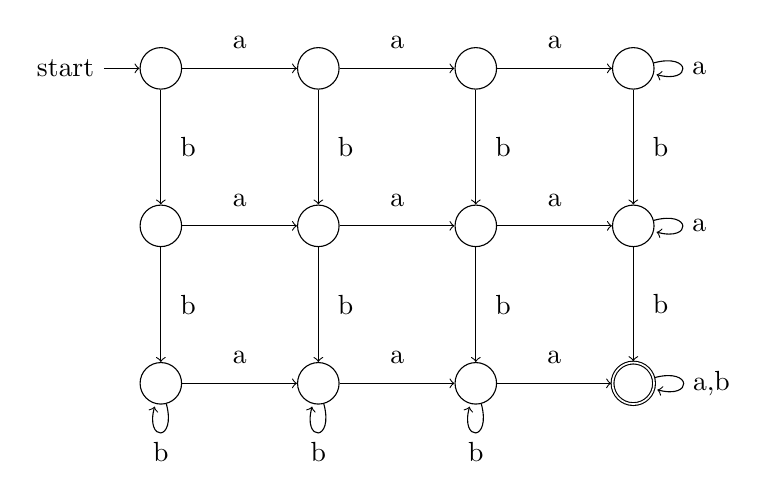
\begin{tikzpicture}

\tikzset{vertex/.style = {shape=circle,draw,minimum size=1.5em}}
\tikzset{edge/.style = {->,> = latex'}}
% vertices
\node[vertex, initial] (1) at  (0,0) {};
\node[vertex] (2) at  (2,0) {};
\node[vertex] (3) at  (4,0) {};
\node[vertex] (4) at (6,0) {};
\node[vertex] (5) at (0,-2) {};
\node[vertex] (6) at (2,-2) {};
\node[vertex] (7) at (4,-2) {};
\node[vertex] (8) at (6,-2) {};
\node[vertex] (9) at (0,-4) {};
\node[vertex] (10) at (2,-4) {};
\node[vertex] (11) at (4,-4) {};
\node[vertex, accepting] (12) at (6,-4) {};

%edges
\draw [->] (1) -- (2) node [midway, label=above: a] {};
\draw [->] (2) -- (3) node [midway, label=above: a] {};
\draw [->] (3) -- (4) node [midway, label=above: a] {};
\draw [->] (5) -- (6) node [midway, label=above: a] {};
\draw [->] (6) -- (7) node [midway, label=above: a] {};
\draw [->] (7) -- (8) node [midway, label=above: a] {};
\draw [->] (9) -- (10) node [midway, label=above: a] {};
\draw [->] (10) -- (11) node [midway, label=above: a] {};
\draw [->] (11) -- (12) node [midway, label=above: a] {};
\draw [->] (1) -- (5) node [midway, label=right: b] {};
\draw [->] (2) -- (6) node [midway, label=right: b] {};
\draw [->] (3) -- (7) node [midway, label=right: b] {};
\draw [->] (4) -- (8) node [midway, label=right: b] {};
\draw [->] (5) -- (9) node [midway, label=right: b] {};
\draw [->] (6) -- (10) node [midway, label=right: b] {};
\draw [->] (7) -- (11) node [midway, label=right: b] {};
\draw [->] (8) -- (12) node [midway, label=right: b] {};
\path (4) edge[loop right] node {a} (4);
\path (8) edge[loop right] node {a} (8);
\path (9) edge[loop below] node {b} (9);
\path (10) edge[loop below] node {b} (10);
\path (11) edge[loop below] node {b} (11);
\path (12) edge[loop right] node {a,b} (12);

\end{tikzpicture}

\noindent1.4c) \\
\noindent Accepts an even number of a's \\
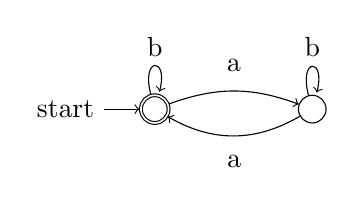
\begin{tikzpicture}

\tikzset{vertex/.style = {shape=circle,draw,minimum size=1em}}
\tikzset{edge/.style = {->,> = latex'}}

% vertices
\node[vertex, initial, accepting] (1) at  (0,0) {};
\node[vertex] (2) at  (2,0) {};

%edges
%\draw [->] (1) -- (2) node [midway, label=above: a] {};
\path [->] (1) edge[bend right=-20] node [label=above: {a}] {} (2);
\draw [->] (2) edge[bend left] node [label=below: {a}] {} (1);
\path (1) edge[loop above] node {b} (1);
\path (2) edge[loop above] node {b} (2);

\end{tikzpicture}
\\
\noindent Accepts one or two b's \\
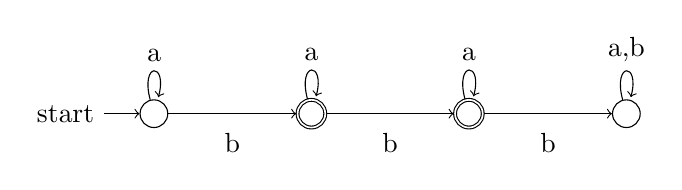
\begin{tikzpicture}

\tikzset{vertex/.style = {shape=circle,draw,minimum size=1em}}
\tikzset{edge/.style = {->,> = latex'}}

% vertices
\node[vertex, initial] (1) at  (0,0) {};
\node[vertex, accepting] (2) at  (2,0) {};
\node[vertex, accepting] (3) at  (4,0) {};
\node[vertex] (4) at  (6,0) {};

%edges
\draw [->] (1) -- (2) node [midway, label=below: b] {};
\draw [->] (2) -- (3) node [midway, label=below: b] {};
\draw [->] (3) -- (4) node [midway, label=below: b] {};
\path (1) edge[loop above] node {a} (1);
\path (2) edge[loop above] node {a} (2);
\path (3) edge[loop above] node {a} (3);
\path (4) edge[loop above] node {a,b} (4);

\end{tikzpicture}

\noindent Accepts even number of a's and one or two b's \\ \\
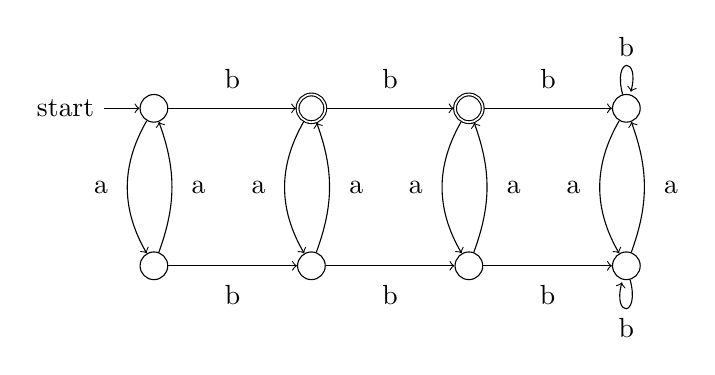
\begin{tikzpicture}

\tikzset{vertex/.style = {shape=circle,draw,minimum size=1em}}
\tikzset{edge/.style = {->,> = latex'}}

% vertices
\node[vertex, initial] (1) at  (0,0) {};
\node[vertex, accepting] (2) at  (2,0) {};
\node[vertex, accepting] (3) at  (4,0) {};
\node[vertex] (4) at  (6,0) {};
\node[vertex] (5) at  (0,-2) {};
\node[vertex] (6) at  (2,-2) {};
\node[vertex] (7) at  (4,-2) {};
\node[vertex] (8) at  (6,-2) {};

%edges
\draw [->] (1) -- (2) node [midway, label=above: b] {};
\draw [->] (2) -- (3) node [midway, label=above: b] {};
\draw [->] (3) -- (4) node [midway, label=above: b] {};
\draw [->] (5) -- (6) node [midway, label=below: b] {};
\draw [->] (6) -- (7) node [midway, label=below: b] {};
\draw [->] (7) -- (8) node [midway, label=below: b] {};
\path [->] (1) edge[bend right] node [label=left: {a}] {} (5);
\path [->] (2) edge[bend right] node [label=left: {a}] {} (6);
\path [->] (3) edge[bend right] node [label=left: {a}] {} (7);
\path [->] (4) edge[bend right] node [label=left: {a}] {} (8);
\path [->] (5) edge[bend left=-20] node [label=right: {a}] {} (1);
\path [->] (6) edge[bend left=-20] node [label=right: {a}] {} (2);
\path [->] (7) edge[bend left=-20] node [label=right: {a}] {} (3);
\path [->] (8) edge[bend left=-20] node [label=right: {a}] {} (4);
\path (4) edge[loop above] node {b} (4);
\path (8) edge[loop below] node {b} (8);

\end{tikzpicture}

\noindent1.4e) \\
Starts with an a \\
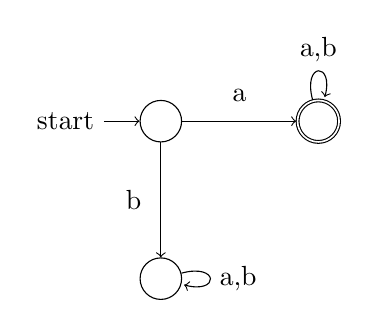
\begin{tikzpicture}

\tikzset{vertex/.style = {shape=circle,draw,minimum size=1.5em}}
\tikzset{edge/.style = {->,> = latex'}}
%verticies
\node[vertex, initial] (1) at  (0,0) {};
\node[vertex, accepting] (2) at  (2,0) {};
\node[vertex] (3) at  (0,-2) {};
%edges
\draw [->] (1) -- (2) node [midway, label=above: a] {};
\draw [->] (1) -- (3) node [midway, label=left: b] {};
\path (2) edge[loop above] node {a,b} (2);
\path (3) edge[loop right] node {a,b} (3);

\end{tikzpicture}

\noindent Has at most one b \\
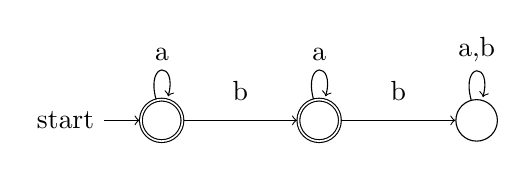
\begin{tikzpicture}

\tikzset{vertex/.style = {shape=circle,draw,minimum size=1.5em}}
\tikzset{edge/.style = {->,> = latex'}}
%verticies
\node[vertex, initial, accepting] (1) at  (0,0) {};
\node[vertex, accepting] (2) at  (2,0) {};
\node[vertex] (3) at  (4,0) {};
%edges
\draw [->] (1) -- (2) node [midway, label=above: b] {};
\draw [->] (2) -- (3) node [midway, label=above: b] {};
\path (1) edge[loop above] node {a} (1);
\path (2) edge[loop above] node {a} (2);
\path (3) edge[loop above] node {a,b} (3);

\end{tikzpicture}

\noindent Starts with an a and has at most one b \\
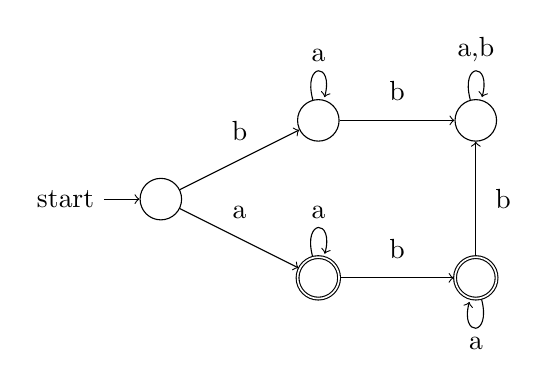
\begin{tikzpicture}

\tikzset{vertex/.style = {shape=circle,draw,minimum size=1.5em}}
\tikzset{edge/.style = {->,> = latex'}}
%verticies
\node[vertex, initial] (1) at  (0,-1) {};
\node[vertex] (2) at  (2,0) {};
\node[vertex] (3) at  (4,0) {};
\node[vertex, accepting] (4) at  (2,-2) {};
\node[vertex, accepting] (5) at  (4,-2) {};
%edges
\draw [->] (1) -- (2) node [midway, label=above: b] {};
\draw [->] (2) -- (3) node [midway, label=above: b] {};
\draw [->] (1) -- (4) node [midway, label=above: a] {};
\draw [->] (4) -- (5) node [midway, label=above: b] {};
\draw [->] (5) -- (3) node [midway, label=right: b] {};
\path (2) edge[loop above] node {a} (2);
\path (3) edge[loop above] node {a,b} (3);
\path (4) edge[loop above] node {a} (4);
\path (5) edge[loop below] node {a} (5);

\end{tikzpicture}

\noindent1.4f) \\
\noindent Has an odd number of a's\\
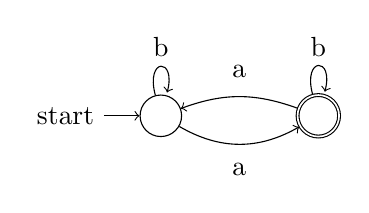
\begin{tikzpicture}

\tikzset{vertex/.style = {shape=circle,draw,minimum size=1.5em}}
\tikzset{edge/.style = {->,> = latex'}}
%verticies
\node[vertex, initial] (1) at  (0,0) {};
\node[vertex, accepting] (2) at  (2,0) {};
%edges
\path [->] (1) edge[bend right] node [label=below: {a}] {} (2);
\path [->] (2) edge[bend left=-20] node [label=above: {a}] {} (1);
\path (1) edge[loop above] node {b} (1);
\path (2) edge[loop above] node {b} (2);

\end{tikzpicture}

\noindent Ends with a b\\
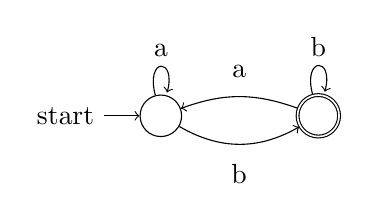
\begin{tikzpicture}

\tikzset{vertex/.style = {shape=circle,draw,minimum size=1.5em}}
\tikzset{edge/.style = {->,> = latex'}}
%verticies
\node[vertex, initial] (1) at  (0,0) {};
\node[vertex, accepting] (2) at  (2,0) {};
%edges
\path [->] (1) edge[bend right] node [label=below: {b}] {} (2);
\path [->] (2) edge[bend left=-20] node [label=above: {a}] {} (1);
\path (1) edge[loop above] node {a} (1);
\path (2) edge[loop above] node {b} (2);

\end{tikzpicture}

\noindent Has an odd number of a's and ends with a b \\
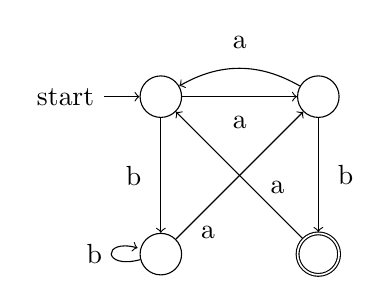
\begin{tikzpicture}

\tikzset{vertex/.style = {shape=circle,draw,minimum size=1.5em}}
\tikzset{edge/.style = {->,> = latex'}}
%verticies
\node[vertex, initial] (1) at  (0,0) {};
\node[vertex] (2) at  (2,0) {};
\node[vertex] (3) at  (0,-2) {};
\node[vertex, accepting] (4) at  (2,-2) {};
%edges
\draw [->] (1) -- (2) node [midway, label=below: a] {};
\draw [->] (1) -- (3) node [midway, label=left: b] {};
\draw [->] (2) -- (4) node [midway, label=right: b] {};
\draw [->] (4) -- (1) node [pos=.2, label=above: a] {};
\draw [->] (3) -- (2) node [pos=.25, label=below: a] {};
\path [->] (2) edge[bend left=-30] node [label=above: {a}] {} (1);
\path (3) edge[loop left] node {b} (3);

\end{tikzpicture}

\noindent1.4g) \\
\noindent Has even length \\
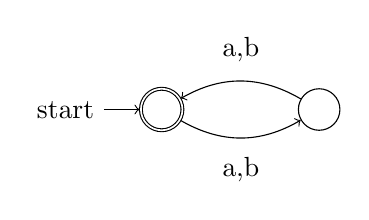
\begin{tikzpicture}

\tikzset{vertex/.style = {shape=circle,draw,minimum size=1.5em}}
\tikzset{edge/.style = {->,> = latex'}}
%verticies
\node[vertex, initial, accepting] (1) at  (0,0) {};
\node[vertex] (2) at  (2,0) {};
%edges
\path [->] (1) edge[bend right] node [label=below: {a,b}] {} (2);
\path [->] (2) edge[bend left=-30] node [label=above: {a,b}] {} (1);
\end{tikzpicture}

\noindent Has an odd number of a's\\
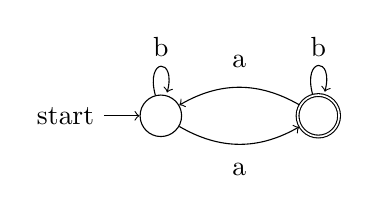
\begin{tikzpicture}

\tikzset{vertex/.style = {shape=circle,draw,minimum size=1.5em}}
\tikzset{edge/.style = {->,> = latex'}}
%verticies
\node[vertex, initial] (1) at  (0,0) {};
\node[vertex, accepting] (2) at  (2,0) {};
%edges
\path [->] (1) edge[bend right] node [label=below: {a}] {} (2);
\path [->] (2) edge[bend left=-30] node [label=above: {a}] {} (1);
\path (1) edge[loop above] node {b} (1);
\path (2) edge[loop above] node {b} (2);

\end{tikzpicture}

\noindent Has even length and an odd number of a's\\
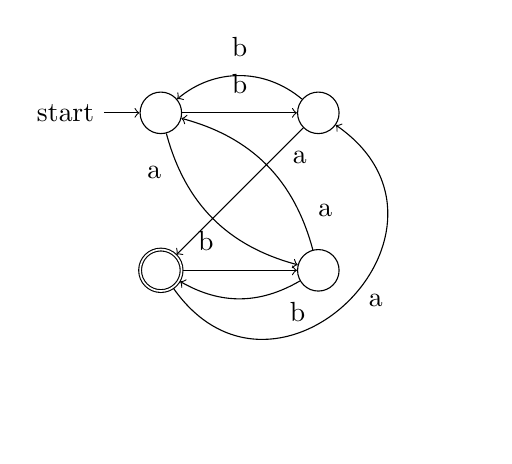
\begin{tikzpicture}

\tikzset{vertex/.style = {shape=circle,draw,minimum size=1.5em}}
\tikzset{edge/.style = {->,> = latex'}}
%verticies
\node[vertex, initial] (1) at  (0,0) {};
\node[vertex] (2) at  (2,0) {};
\node[vertex, accepting] (3) at  (0,-2) {};
\node[vertex] (4) at  (2,-2) {};
%edges
\draw [->] (1) -- (2) node [midway, label=above: b] {};
\draw [->] (3) -- (4) node [midway, label=above: b, pos=.2] {};
\draw [->] (2) -- (3) node [pos=.03, label=below: a] {};
\path [->] (2) edge[bend left=-40] node [label=above: {b}] {} (1);
\path [->] (1) edge[bend right] node [label=left: {a}, pos=.2] {} (4);
\path [->] (4) edge[bend left] node [label=below: {b}, pos=.02] {} (3);
\path [->] (4) edge[bend left=-30] node [label=right: {a}, pos=.2] {} (1);
\path [->, looseness=2] (3) edge[bend right=100] node [label=right: {a}] {} (2);

\end{tikzpicture}

\noindent1.5c)\\
\noindent Contains the substring ab or ba \\
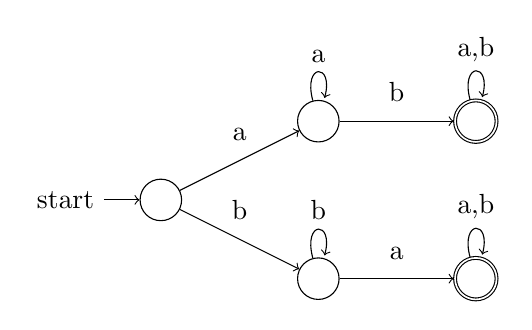
\begin{tikzpicture}

\tikzset{vertex/.style = {shape=circle,draw,minimum size=1.5em}}
\tikzset{edge/.style = {->,> = latex'}}
%verticies
\node[vertex, initial] (1) at  (0,-1) {};
\node[vertex] (2) at  (2,0) {};
\node[vertex, accepting] (3) at  (4,0) {};
\node[vertex] (4) at  (2,-2) {};
\node[vertex, accepting] (5) at  (4,-2) {};
%edges
\draw [->] (1) -- (2) node [midway, label=above: a] {};
\draw [->] (2) -- (3) node [midway, label=above: b] {};
\draw [->] (1) -- (4) node [midway, label=above: b] {};
\draw [->] (4) -- (5) node [midway, label=above: a] {};
\path (2) edge[loop above] node {a} (2);
\path (3) edge[loop above] node {a,b} (3);
\path (4) edge[loop above] node {b} (4);
\path (5) edge[loop above] node {a,b} (5);

\end{tikzpicture}

\noindent Does not contain the substring ab or ba \\
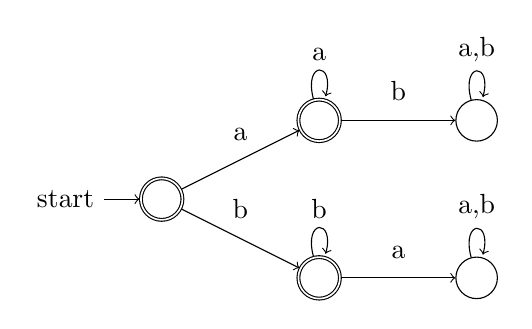
\begin{tikzpicture}

\tikzset{vertex/.style = {shape=circle,draw,minimum size=1.5em}}
\tikzset{edge/.style = {->,> = latex'}}
%verticies
\node[vertex, initial, accepting] (1) at  (0,-1) {};
\node[vertex, accepting] (2) at  (2,0) {};
\node[vertex] (3) at  (4,0) {};
\node[vertex, accepting] (4) at  (2,-2) {};
\node[vertex] (5) at  (4,-2) {};
%edges
\draw [->] (1) -- (2) node [midway, label=above: a] {};
\draw [->] (2) -- (3) node [midway, label=above: b] {};
\draw [->] (1) -- (4) node [midway, label=above: b] {};
\draw [->] (4) -- (5) node [midway, label=above: a] {};
\path (2) edge[loop above] node {a} (2);
\path (3) edge[loop above] node {a,b} (3);
\path (4) edge[loop above] node {b} (4);
\path (5) edge[loop above] node {a,b} (5);

\end{tikzpicture}

\noindent1.5d) \\
\noindent Any string in a*b* \\
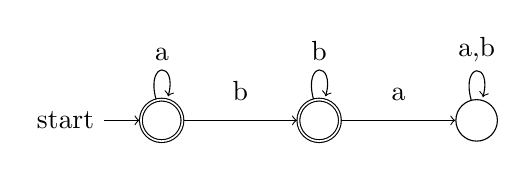
\begin{tikzpicture}

\tikzset{vertex/.style = {shape=circle,draw,minimum size=1.5em}}
\tikzset{edge/.style = {->,> = latex'}}
%verticies
\node[vertex, initial, accepting] (1) at  (0,0) {};
\node[vertex, accepting] (2) at  (2,0) {};
\node[vertex] (3) at  (4,0) {};
%edges
\draw [->] (1) -- (2) node [midway, label=above: b] {};
\draw [->] (2) -- (3) node [midway, label=above: a] {};
\path (1) edge[loop above] node {a} (1);
\path (2) edge[loop above] node {b} (2);
\path (3) edge[loop above] node {a,b} (3);

\end{tikzpicture}

\noindent Any string not in a*b* \\
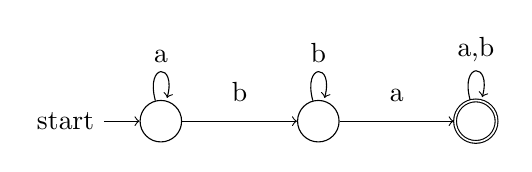
\begin{tikzpicture}

\tikzset{vertex/.style = {shape=circle,draw,minimum size=1.5em}}
\tikzset{edge/.style = {->,> = latex'}}
%verticies
\node[vertex, initial] (1) at  (0,0) {};
\node[vertex] (2) at  (2,0) {};
\node[vertex, accepting] (3) at  (4,0) {};
%edges
\draw [->] (1) -- (2) node [midway, label=above: b] {};
\draw [->] (2) -- (3) node [midway, label=above: a] {};
\path (1) edge[loop above] node {a} (1);
\path (2) edge[loop above] node {b} (2);
\path (3) edge[loop above] node {a,b} (3);

\end{tikzpicture}

\noindent1.5e)
\noindent Any string in (ab+)*\\
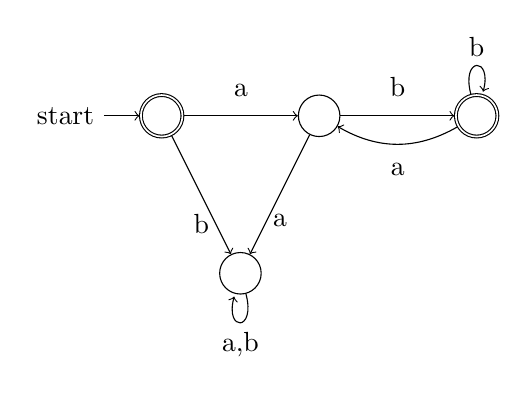
\begin{tikzpicture}

\tikzset{vertex/.style = {shape=circle,draw,minimum size=1.5em}}
\tikzset{edge/.style = {->,> = latex'}}
%verticies
\node[vertex, initial, accepting] (1) at  (0,0) {};
\node[vertex] (2) at  (2,0) {};
\node[vertex, accepting] (3) at  (4,0) {};
\node[vertex] (4) at  (1,-2) {};
%edges
\draw [->] (1) -- (2) node [midway, label=above: a] {};
\draw [->] (2) -- (3) node [midway, label=above: b] {};
\draw [->] (1) -- (4) node [midway, label=below: b] {};
\draw [->] (2) -- (4) node [midway, label=below: a] {};
\path [->] (3) edge[bend left] node [label=below: {a}] {} (2);
\path (3) edge[loop above] node {b} (3);
\path (4) edge[loop below] node {a,b} (4);

\end{tikzpicture}

\noindent Any string not in (ab+)*\\
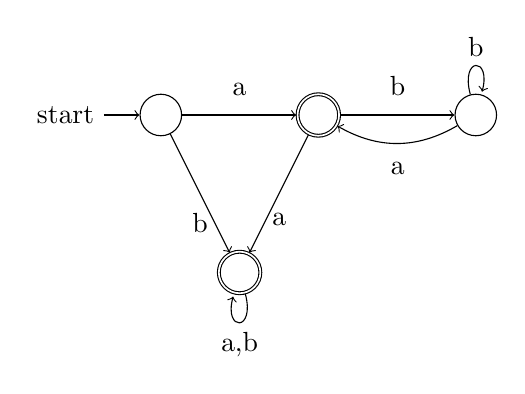
\begin{tikzpicture}

\tikzset{vertex/.style = {shape=circle,draw,minimum size=1.5em}}
\tikzset{edge/.style = {->,> = latex'}}
%verticies
\node[vertex, initial] (1) at  (0,0) {};
\node[vertex, accepting] (2) at  (2,0) {};
\node[vertex] (3) at  (4,0) {};
\node[vertex, accepting] (4) at  (1,-2) {};
%edges
\draw [->] (1) -- (2) node [midway, label=above: a] {};
\draw [->] (2) -- (3) node [midway, label=above: b] {};
\draw [->] (1) -- (4) node [midway, label=below: b] {};
\draw [->] (2) -- (4) node [midway, label=below: a] {};
\path [->] (3) edge[bend left] node [label=below: {a}] {} (2);
\path (3) edge[loop above] node {b} (3);
\path (4) edge[loop below] node {a,b} (4);

\end{tikzpicture}

\noindent Any string in a*$\cup$b*\\
\begin{tikzpicture}

\tikzset{vertex/.style = {shape=circle,draw,minimum size=1.5em}}
\tikzset{edge/.style = {->,> = latex'}}
%verticies
\node[vertex, initial, accepting] (1) at  (0,-2) {};
\node[vertex, accepting] (2) at  (2,0) {};
\node[vertex] (3) at  (4,-2) {};
\node[vertex, accepting] (4) at  (2,-4) {};
%edges
\draw [->] (1) -- (2) node [midway, label=above: a] {};
\draw [->] (2) -- (3) node [midway, label=above: b] {};
\draw [->] (1) -- (4) node [midway, label=below: b] {};
\draw [->] (4) -- (3) node [midway, label=below: a] {};
%\path [->] (3) edge[bend left] node [label=below: {a}] {} (2);
\path (2) edge[loop above] node {a} (2);
\path (3) edge[loop right] node {a,b} (3);
\path (4) edge[loop below] node {b} (4);

\end{tikzpicture}

\noindent Any string not in a*$\cup$b*\\
\begin{tikzpicture}

\tikzset{vertex/.style = {shape=circle,draw,minimum size=1.5em}}
\tikzset{edge/.style = {->,> = latex'}}
%verticies
\node[vertex, initial] (1) at  (0,-2) {};
\node[vertex] (2) at  (2,0) {};
\node[vertex, accepting] (3) at  (4,-2) {};
\node[vertex] (4) at  (2,-4) {};
%edges
\draw [->] (1) -- (2) node [midway, label=above: a] {};
\draw [->] (2) -- (3) node [midway, label=above: b] {};
\draw [->] (1) -- (4) node [midway, label=below: b] {};
\draw [->] (4) -- (3) node [midway, label=below: a] {};
%\path [->] (3) edge[bend left] node [label=below: {a}] {} (2);
\path (2) edge[loop above] node {a} (2);
\path (3) edge[loop right] node {a,b} (3);
\path (4) edge[loop below] node {b} (4);

\end{tikzpicture}

\noindent1.5g) \\
\noindent Accepts exactly two a's \\

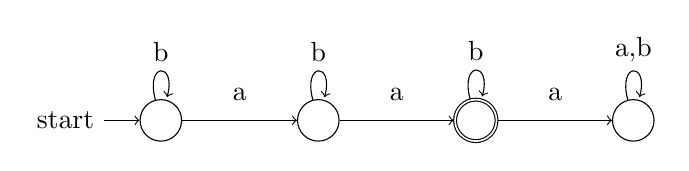
\begin{tikzpicture}

\tikzset{vertex/.style = {shape=circle,draw,minimum size=1.5em}}
\tikzset{edge/.style = {->,> = latex'}}
%verticies
\node[vertex, initial] (1) at  (0,0) {};
\node[vertex] (2) at  (2,0) {};
\node[vertex, accepting] (3) at  (4,0) {};
\node[vertex] (4) at  (6,0) {};
%edges
\draw [->] (1) -- (2) node [midway, label=above: a] {};
\draw [->] (2) -- (3) node [midway, label=above: a] {};
\draw [->] (3) -- (4) node [midway, label=above: a] {};
\path (1) edge[loop above] node {b} (1);
\path (2) edge[loop above] node {b} (2);
\path (3) edge[loop above] node {b} (3);
\path (4) edge[loop above] node {a,b} (4);

\end{tikzpicture}

\noindent Accepts strings not containing exactly two a's \\

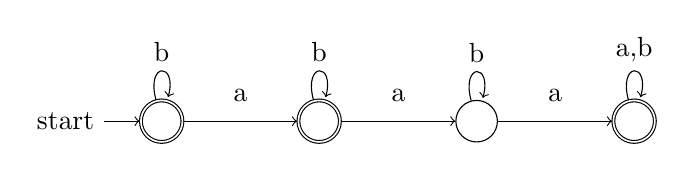
\begin{tikzpicture}

\tikzset{vertex/.style = {shape=circle,draw,minimum size=1.5em}}
\tikzset{edge/.style = {->,> = latex'}}
%verticies
\node[vertex, initial, accepting] (1) at  (0,0) {};
\node[vertex, accepting] (2) at  (2,0) {};
\node[vertex] (3) at  (4,0) {};
\node[vertex, accepting] (4) at  (6,0) {};
%edges
\draw [->] (1) -- (2) node [midway, label=above: a] {};
\draw [->] (2) -- (3) node [midway, label=above: a] {};
\draw [->] (3) -- (4) node [midway, label=above: a] {};
\path (1) edge[loop above] node {b} (1);
\path (2) edge[loop above] node {b} (2);
\path (3) edge[loop above] node {b} (3);
\path (4) edge[loop above] node {a,b} (4);

\end{tikzpicture}

\noindent1.5h) \\
\noindent Any string except a and b \\

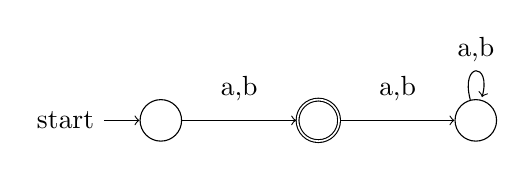
\begin{tikzpicture}

\tikzset{vertex/.style = {shape=circle,draw,minimum size=1.5em}}
\tikzset{edge/.style = {->,> = latex'}}
%verticies
\node[vertex, initial] (1) at  (0,0) {};
\node[vertex, accepting] (2) at  (2,0) {};
\node[vertex] (3) at  (4,0) {};
%edges
\draw [->] (1) -- (2) node [midway, label=above: {a,b}] {};
\draw [->] (2) -- (3) node [midway, label=above: {a,b}] {};
\path (3) edge[loop above] node {a,b} (3);

\end{tikzpicture}

\noindent Any string that is a and b \\

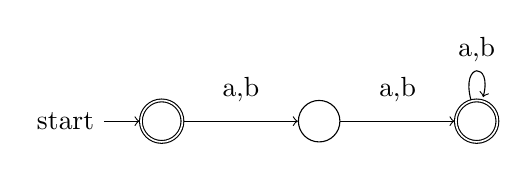
\begin{tikzpicture}

\tikzset{vertex/.style = {shape=circle,draw,minimum size=1.5em}}
\tikzset{edge/.style = {->,> = latex'}}
%verticies
\node[vertex, initial, accepting] (1) at  (0,0) {};
\node[vertex] (2) at  (2,0) {};
\node[vertex, accepting] (3) at  (4,0) {};
%edges
\draw [->] (1) -- (2) node [midway, label=above: {a,b}] {};
\draw [->] (2) -- (3) node [midway, label=above: {a,b}] {};
\path (3) edge[loop above] node {a,b} (3);

\end{tikzpicture}

\noindent1.6a) \\
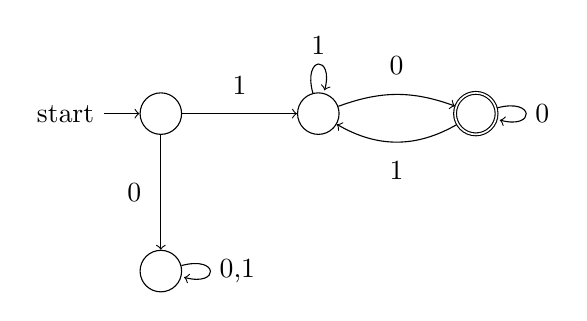
\begin{tikzpicture}

\tikzset{vertex/.style = {shape=circle,draw,minimum size=1.5em}}
\tikzset{edge/.style = {->,> = latex'}}
%verticies
\node[vertex, initial] (1) at  (0,0) {};
\node[vertex] (2) at  (2,0) {};
\node[vertex, accepting] (3) at  (4,0) {};
\node[vertex] (4) at  (0,-2) {};
%edges
\draw [->] (1) -- (2) node [midway, label=above: 1] {};
\draw [->] (1) -- (4) node [midway, label=left: 0] {};
\path [->] (3) edge[bend left] node [label=below: {1}] {} (2);
\path [->] (2) edge[bend right=-20] node [label=above: {0}] {} (3);
\path (2) edge[loop above] node {1} (2);
\path (3) edge[loop right] node {0} (3);
\path (4) edge[loop right] node {0,1} (4);

\end{tikzpicture}

\noindent1.6b) \\
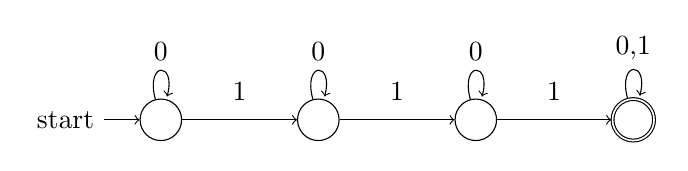
\begin{tikzpicture}

\tikzset{vertex/.style = {shape=circle,draw,minimum size=1.5em}}
\tikzset{edge/.style = {->,> = latex'}}
%verticies
\node[vertex, initial] (1) at  (0,0) {};
\node[vertex] (2) at  (2,0) {};
\node[vertex] (3) at  (4,0) {};
\node[vertex, accepting] (4) at  (6,0) {};
%edges
\draw [->] (1) -- (2) node [midway, label=above: 1] {};
\draw [->] (2) -- (3) node [midway, label=above: 1] {};
\draw [->] (3) -- (4) node [midway, label=above: 1] {};
\path (1) edge[loop above] node {0} (1);
\path (2) edge[loop above] node {0} (2);
\path (3) edge[loop above] node {0} (3);
\path (4) edge[loop above] node {0,1} (4);

\end{tikzpicture}

\noindent1.6c) \\
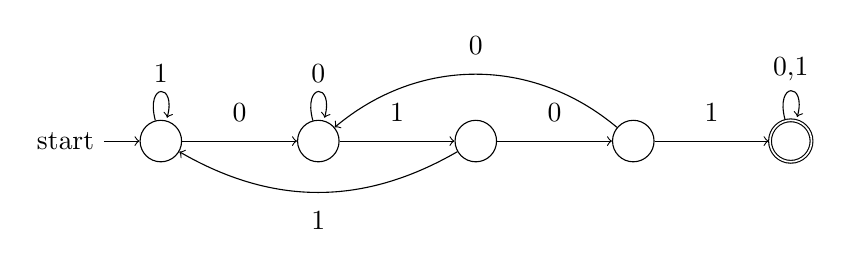
\begin{tikzpicture}

\tikzset{vertex/.style = {shape=circle,draw,minimum size=1.5em}}
\tikzset{edge/.style = {->,> = latex'}}
%verticies
\node[vertex, initial] (1) at  (0,0) {};
\node[vertex] (2) at  (2,0) {};
\node[vertex] (3) at  (4,0) {};
\node[vertex] (4) at  (6,0) {};
\node[vertex, accepting] (5) at  (8,0) {};
%edges
\draw [->] (1) -- (2) node [midway, label=above: 0] {};
\draw [->] (2) -- (3) node [midway, label=above: 1] {};
\draw [->] (3) -- (4) node [midway, label=above: 0] {};
\draw [->] (4) -- (5) node [midway, label=above: 1] {};
\path [->] (4) edge[bend left=-40] node [label=above: {0}] {} (2);
\path [->] (3) edge[bend left] node [label=below: {1}] {} (1);
\path (1) edge[loop above] node {1} (1);
\path (2) edge[loop above] node {0} (2);
\path (5) edge[loop above] node {0,1} (5);

\end{tikzpicture}

\noindent1.6d) \\
\begin{tikzpicture}

\tikzset{vertex/.style = {shape=circle,draw,minimum size=1.5em}}
\tikzset{edge/.style = {->,> = latex'}}
%verticies
\node[vertex, initial] (1) at  (0,0) {};
\node[vertex] (2) at  (2,0) {};
\node[vertex, accepting] (3) at  (4,0) {};
\node[vertex, accepting] (4) at  (6,0) {};
\node[vertex] (5) at  (4,-2) {};
%edges
\draw [->] (1) -- (2) node [midway, label=above: {0,1}] {};
\draw [->] (2) -- (3) node [midway, label=above: {0,1}] {};
\draw [->] (3) -- (4) node [midway, label=above: 0] {};
\draw [->] (3) -- (5) node [midway, label=right: 1] {};
\path (5) edge[loop below] node {0,1} (5);
\path (4) edge[loop above] node {0,1} (4);

\end{tikzpicture}

\noindent1.6e) \\
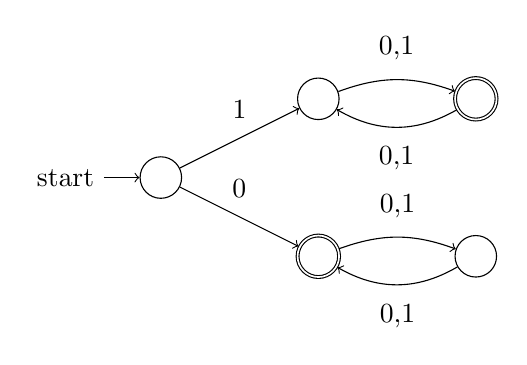
\begin{tikzpicture}

\tikzset{vertex/.style = {shape=circle,draw,minimum size=1.5em}}
\tikzset{edge/.style = {->,> = latex'}}
%verticies
\node[vertex, initial] (1) at  (0,-1) {};
\node[vertex] (2) at  (2,0) {};
\node[vertex, accepting] (3) at  (4,0) {};
\node[vertex, accepting] (4) at  (2,-2) {};
\node[vertex] (5) at  (4,-2) {};
%edges
\draw [->] (1) -- (2) node [midway, label=above: 1] {};
\draw [->] (1) -- (4) node [midway, label=above: 0] {};
\path [->] (2) edge[bend right=-20] node [label=above: {0,1}] {} (3);
\path [->] (3) edge[bend left] node [label=below: {0,1}] {} (2);
\path [->] (4) edge[bend right=-20] node [label=above: {0,1}] {} (5);
\path [->] (5) edge[bend left] node [label=below: {0,1}] {} (4);

\end{tikzpicture}

\noindent1.6f) \\
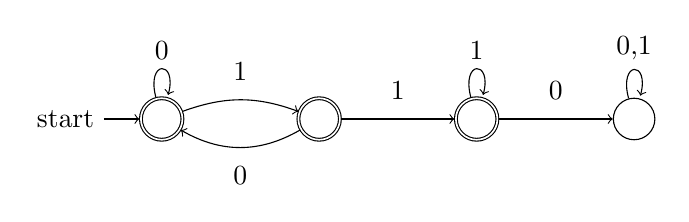
\begin{tikzpicture}

\tikzset{vertex/.style = {shape=circle,draw,minimum size=1.5em}}
\tikzset{edge/.style = {->,> = latex'}}
%verticies
\node[vertex, initial, accepting] (1) at  (0,0) {};
\node[vertex, accepting] (2) at  (2,0) {};
\node[vertex, accepting] (3) at  (4,0) {};
\node[vertex] (4) at  (6,0) {};
%edges
\draw [->] (2) -- (3) node [midway, label=above: {1}] {};
\draw [->] (3) -- (4) node [midway, label=above: {0}] {};
\path [->] (1) edge[bend right=-20] node [label=above: {1}] {} (2);
\path [->] (2) edge[bend left] node [label=below: {0}] {} (1);
\path (1) edge[loop above] node {0} (1);
\path (3) edge[loop above] node {1} (3);
\path (4) edge[loop above] node {0,1} (4);

\end{tikzpicture}

\noindent1.6g) \\
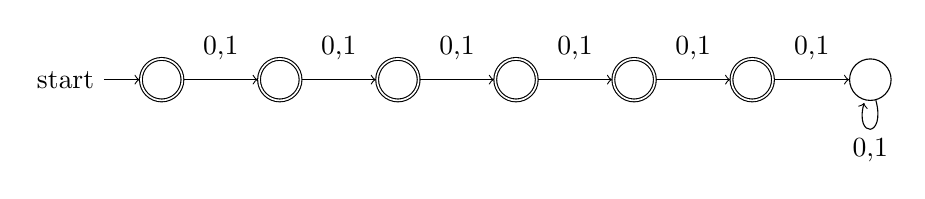
\begin{tikzpicture}

\tikzset{vertex/.style = {shape=circle,draw,minimum size=1.5em}}
\tikzset{edge/.style = {->,> = latex'}}
%verticies
\node[vertex, initial, accepting] (1) at  (0,0) {};
\node[vertex, accepting] (2) at  (1.5,0) {};
\node[vertex, accepting] (3) at  (3,0) {};
\node[vertex, accepting] (4) at  (4.5,0) {};
\node[vertex, accepting] (5) at  (6,0) {};
\node[vertex, accepting] (6) at  (7.5,0) {};
\node[vertex] (7) at  (9,0) {};
%edges
\draw [->] (2) -- (3) node [midway, label=above: {0,1}] {};
\draw [->] (3) -- (4) node [midway, label=above: {0,1}] {};
\draw [->] (4) -- (5) node [midway, label=above: {0,1}] {};
\draw [->] (5) -- (6) node [midway, label=above: {0,1}] {};
\draw [->] (6) -- (7) node [midway, label=above: {0,1}] {};
\draw [->] (1) -- (2) node [midway, label=above: {0,1}] {};
\path (7) edge[loop below] node {0,1} (7);

\end{tikzpicture}

\noindent1.6h) \\
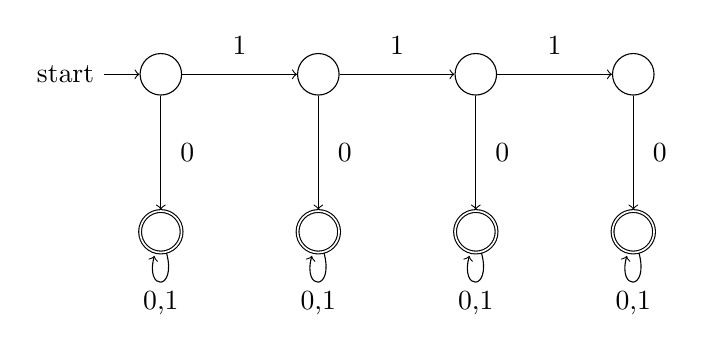
\begin{tikzpicture}

\tikzset{vertex/.style = {shape=circle,draw,minimum size=1.5em}}
\tikzset{edge/.style = {->,> = latex'}}
%verticies
\node[vertex, initial] (1) at  (0,0) {};
\node[vertex] (2) at  (2,0) {};
\node[vertex] (3) at  (4,0) {};
\node[vertex] (4) at  (6,0) {};
\node[vertex, accepting] (5) at  (0,-2) {};
\node[vertex, accepting] (6) at  (2,-2) {};
\node[vertex, accepting] (7) at  (4,-2) {};
\node[vertex, accepting] (8) at  (6,-2) {};
%edges
\draw [->] (1) -- (2) node [midway, label=above: {1}] {};
\draw [->] (2) -- (3) node [midway, label=above: {1}] {};
\draw [->] (3) -- (4) node [midway, label=above: {1}] {};
\draw [->] (1) -- (5) node [midway, label=right: {0}] {};
\draw [->] (2) -- (6) node [midway, label=right: {0}] {};
\draw [->] (3) -- (7) node [midway, label=right: {0}] {};
\draw [->] (4) -- (8) node [midway, label=right: {0}] {};
\path (5) edge[loop below] node {0,1} (5);
\path (6) edge[loop below] node {0,1} (6);
\path (7) edge[loop below] node {0,1} (7);
\path (8) edge[loop below] node {0,1} (8);

\end{tikzpicture}

\noindent1.6i) \\
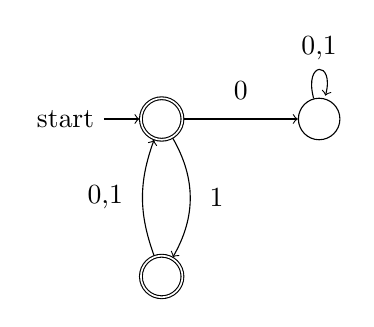
\begin{tikzpicture}

\tikzset{vertex/.style = {shape=circle,draw,minimum size=1.5em}}
\tikzset{edge/.style = {->,> = latex'}}
%verticies
\node[vertex, initial, accepting] (1) at  (0,0) {};
\node[vertex] (2) at  (2,0) {};
\node[vertex, accepting] (3) at  (0,-2) {};
\draw [->] (1) -- (2) node [midway, label=above: {0}] {};
\path [->] (1) edge[bend left] node [label=right: {1}] {} (3);
\path [->] (3) edge[bend right=-20] node [label=left: {0,1}] {} (1);
\path (2) edge[loop above] node {0,1} (2);

\end{tikzpicture}

\noindent1.6j) \\
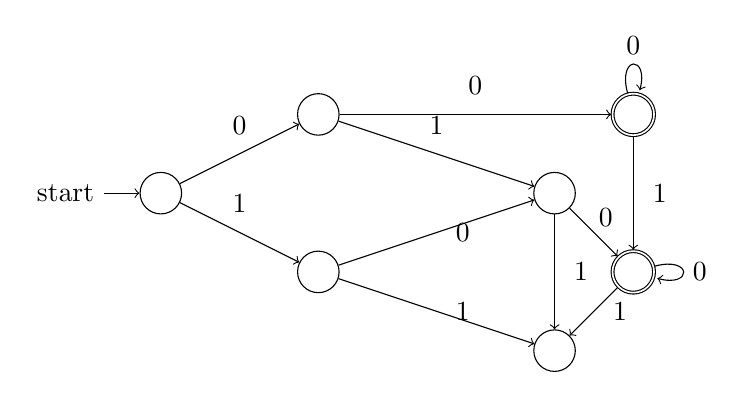
\begin{tikzpicture}

\tikzset{vertex/.style = {shape=circle,draw,minimum size=1.5em}}
\tikzset{edge/.style = {->,> = latex'}}
%verticies
\node[vertex, initial] (1) at  (0,-1) {};
\node[vertex] (2) at  (2,0) {};
\node[vertex, accepting] (3) at  (6,0) {};
\node[vertex] (4) at  (5,-1) {};
\node[vertex] (5) at  (2,-2) {};
\node[vertex] (6) at  (5,-3) {};
\node[vertex, accepting] (7) at  (6,-2) {};
%edges
\draw [->] (1) -- (2) node [midway, label=above: {0}] {};
\draw [->] (1) -- (5) node [midway, label=above: {1}] {};
\draw [->] (2) -- (3) node [midway, label=above: {0}] {};
\draw [->] (2) -- (4) node [midway, label=above: {1}] {};
\draw [->] (3) -- (7) node [midway, label=right: {1}] {};
\draw [->] (5) -- (4) node [midway, label=right: {0}] {};
\draw [->] (4) -- (7) node [midway, label=right: {0}, pos=0.2] {};
\draw [->] (4) -- (6) node [midway, label=right: {1}] {};
\draw [->] (5) -- (6) node [midway, label=right: {1}] {};
\draw [->] (7) -- (6) node [midway, label=right: {1}] {};
\path (3) edge[loop above] node {0} (3);
\path (7) edge[loop right] node {0} (7);

\end{tikzpicture}

\noindent1.6k) \\
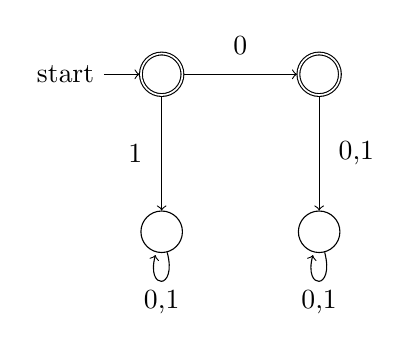
\begin{tikzpicture}

\tikzset{vertex/.style = {shape=circle,draw,minimum size=1.5em}}
\tikzset{edge/.style = {->,> = latex'}}
%verticies
\node[vertex, initial, accepting] (1) at  (0,0) {};
\node[vertex, accepting] (2) at  (2,0) {};
\node[vertex] (3) at  (0,-2) {};
\node[vertex] (4) at  (2,-2) {};
\draw [->] (1) -- (2) node [midway, label=above: {0}] {};
\draw [->] (1) -- (3) node [midway, label=left: {1}] {};
\draw [->] (2) -- (4) node [midway, label=right: {0,1}] {};
\path (3) edge[loop below] node {0,1} (3);
\path (4) edge[loop below] node {0,1} (4);

\end{tikzpicture}

\noindent1.6l) \\
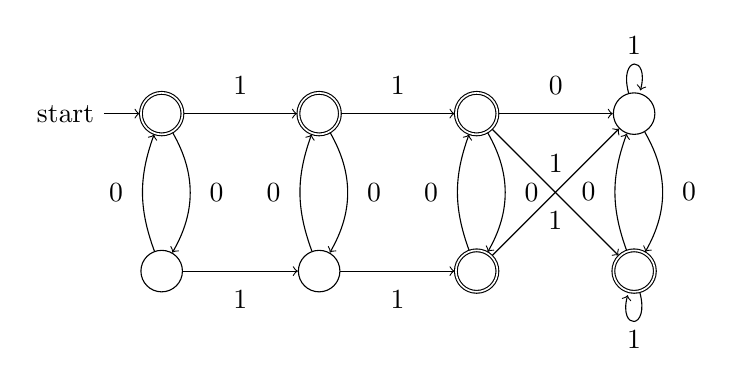
\begin{tikzpicture}

\tikzset{vertex/.style = {shape=circle,draw,minimum size=1.5em}}
\tikzset{edge/.style = {->,> = latex'}}
%verticies
\node[vertex, initial, accepting] (1) at  (0,0) {};
\node[vertex, accepting] (2) at  (2,0) {};
\node[vertex, accepting] (3) at  (4,0) {};
\node[vertex] (4) at  (6,0) {};
\node[vertex] (5) at  (0,-2) {};
\node[vertex] (6) at  (2,-2) {};
\node[vertex, accepting] (7) at  (4,-2) {};
\node[vertex, accepting] (8) at  (6,-2) {};
\draw [->] (1) -- (2) node [midway, label=above: {1}] {};
\draw [->] (2) -- (3) node [midway, label=above: {1}] {};
\draw [->] (3) -- (4) node [midway, label=above: {0}] {};
\draw [->] (5) -- (6) node [midway, label=below: {1}] {};
\draw [->] (6) -- (7) node [midway, label=below: {1}] {};
\draw [->] (3) -- (8) node [midway, label=below: {1}] {};
\draw [->] (7) -- (4) node [midway, label=above: {1}] {};
\path [->] (1) edge[bend left] node [label=right: {0}] {} (5);
\path [->] (5) edge[bend right=-20] node [label=left: {0}] {} (1);
\path [->] (2) edge[bend left] node [label=right: {0}] {} (6);
\path [->] (6) edge[bend right=-20] node [label=left: {0}] {} (2);
\path [->] (3) edge[bend left] node [label=right: {0}] {} (7);
\path [->] (7) edge[bend right=-20] node [label=left: {0}] {} (3);
\path [->] (4) edge[bend left] node [label=right: {0}] {} (8);
\path [->] (8) edge[bend right=-20] node [label=left: {0}] {} (4);
\path (4) edge[loop above] node {1} (4);
\path (8) edge[loop below] node {1} (8);

\end{tikzpicture}

\noindent1.6m) \\
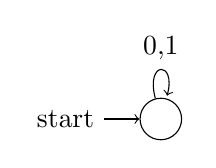
\begin{tikzpicture}

\tikzset{vertex/.style = {shape=circle,draw,minimum size=1.5em}}
\tikzset{edge/.style = {->,> = latex'}}
%verticies
\node[vertex, initial] (1) at  (0,0) {};
\path (1) edge[loop above] node {0,1} (1);

\end{tikzpicture}

\noindent1.6n) \\
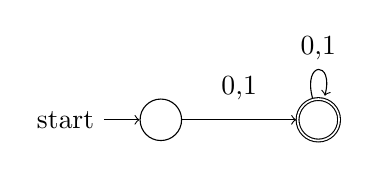
\begin{tikzpicture}

\tikzset{vertex/.style = {shape=circle,draw,minimum size=1.5em}}
\tikzset{edge/.style = {->,> = latex'}}
%verticies
\node[vertex, initial] (1) at  (0,0) {};
\node[vertex, accepting] (2) at  (2,0) {};
\draw [->] (1) -- (2) node [midway, label=above: {0,1}] {};
\path (2) edge[loop above] node {0,1} (2);

\end{tikzpicture}

\noindent1.7b) \\
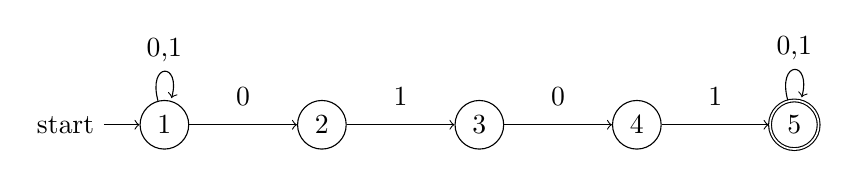
\begin{tikzpicture}

\tikzset{vertex/.style = {shape=circle,draw,minimum size=1.5em}}
\tikzset{edge/.style = {->,> = latex'}}
%verticies
\node[vertex, initial] (1) at  (0,0) {1};
\node[vertex] (2) at  (2,0) {2};
\node[vertex] (3) at  (4,0) {3};
\node[vertex] (4) at  (6,0) {4};
\node[vertex, accepting] (5) at  (8,0) {5};
\draw [->] (1) -- (2) node [midway, label=above: {0}] {};
\draw [->] (2) -- (3) node [midway, label=above: {1}] {};
\draw [->] (3) -- (4) node [midway, label=above: {0}] {};
\draw [->] (4) -- (5) node [midway, label=above: {1}] {};
%\path [->] (1) edge[bend left] node [label=right: {0}] {} (5);
\path (1) edge[loop above] node {0,1} (1);
\path (5) edge[loop above] node {0,1} (5);

\end{tikzpicture}

\noindent1.7c) \\
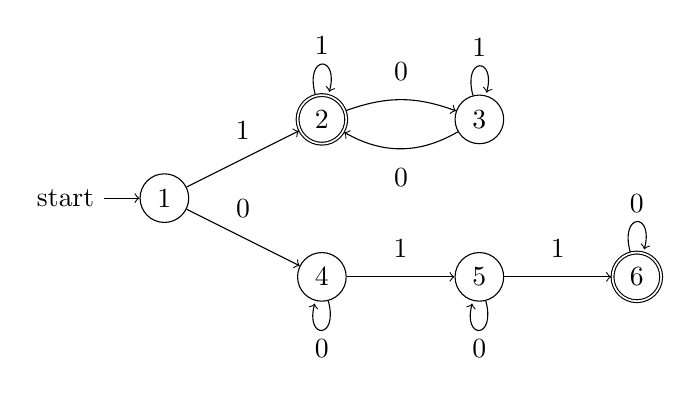
\begin{tikzpicture}

\tikzset{vertex/.style = {shape=circle,draw,minimum size=1.5em}}
\tikzset{edge/.style = {->,> = latex'}}
%verticies
\node[vertex, initial] (1) at  (0,-1) {1};
\node[vertex, accepting] (2) at  (2,0) {2};
\node[vertex] (3) at  (4,0) {3};
\node[vertex] (4) at  (2,-2) {4};
\node[vertex] (5) at  (4,-2) {5};
\node[vertex, accepting] (6) at  (6,-2) {6};
\draw [->] (1) -- (2) node [midway, label=above: {1}] {};
\draw [->] (1) -- (4) node [midway, label=above: {0}] {};
\draw [->] (4) -- (5) node [midway, label=above: {1}] {};
\draw [->] (5) -- (6) node [midway, label=above: {1}] {};
\path [->] (3) edge[bend left] node [label=below: {0}] {} (2);
\path [->] (2) edge[bend right=-20] node [label=above: {0}] {} (3);
\path (2) edge[loop above] node {1} (2);
\path (3) edge[loop above] node {1} (3);
\path (4) edge[loop below] node {0} (4);
\path (5) edge[loop below] node {0} (5);
\path (6) edge[loop above] node {0} (6);

\end{tikzpicture}

\noindent1.7d) \\
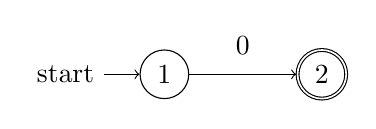
\begin{tikzpicture}

\tikzset{vertex/.style = {shape=circle,draw,minimum size=1.5em}}
\tikzset{edge/.style = {->,> = latex'}}
%verticies
\node[vertex, initial] (1) at  (0,0) {1};
\node[vertex, accepting] (2) at  (2,0) {2};
\draw [->] (1) -- (2) node [midway, label=above: {0}] {};
%\path [->] (3) edge[bend left] node [label=below: {0}] {} (2);
%\path [->] (2) edge[bend right=-20] node [label=above: {0}] {} (3);
%\path (2) edge[loop above] node {1} (2);

\end{tikzpicture}

\noindent1.7e) \\
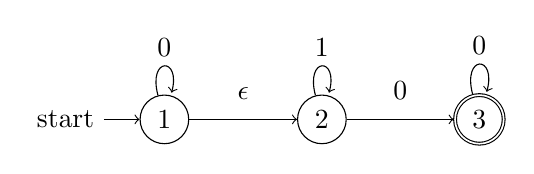
\begin{tikzpicture}

\tikzset{vertex/.style = {shape=circle,draw,minimum size=1.5em}}
\tikzset{edge/.style = {->,> = latex'}}
%verticies
\node[vertex, initial] (1) at  (0,0) {1};
\node[vertex] (2) at  (2,0) {2};
\node[vertex, accepting] (3) at  (4,0) {3};
\draw [->] (1) -- (2) node [midway, label=above: {$\epsilon$}] {};
\draw [->] (2) -- (3) node [midway, label=above: {0}] {};
%\path [->] (3) edge[bend left] node [label=below: {0}] {} (2);
%\path [->] (2) edge[bend right=-20] node [label=above: {0}] {} (3);
\path (1) edge[loop above] node {0} (1);
\path (2) edge[loop above] node {1} (2);
\path (3) edge[loop above] node {0} (3);

\end{tikzpicture}

\noindent1.7g) \\
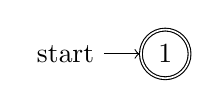
\begin{tikzpicture}

\tikzset{vertex/.style = {shape=circle,draw,minimum size=1.5em}}
\tikzset{edge/.style = {->,> = latex'}}
%verticies
\node[vertex, initial, accepting] (1) at  (0,0) {1};
%\draw [->] (1) -- (2) node [midway, label=above: {$\epsilon$}] {};
%\path [->] (3) edge[bend left] node [label=below: {0}] {} (2);
%\path [->] (2) edge[bend right=-20] node [label=above: {0}] {} (3);
%\path (1) edge[loop above] node {0} (1);

\end{tikzpicture}

\noindent1.7h) \\
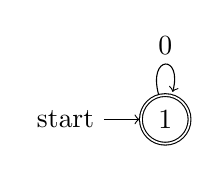
\begin{tikzpicture}

\tikzset{vertex/.style = {shape=circle,draw,minimum size=1.5em}}
\tikzset{edge/.style = {->,> = latex'}}
%verticies
\node[vertex, initial, accepting] (1) at  (0,0) {1};
%\draw [->] (1) -- (2) node [midway, label=above: {$\epsilon$}] {};
%\path [->] (3) edge[bend left] node [label=below: {0}] {} (2);
%\path [->] (2) edge[bend right=-20] node [label=above: {0}] {} (3);
\path (1) edge[loop above] node {0} (1);

\end{tikzpicture}

\noindent1.8a) \\
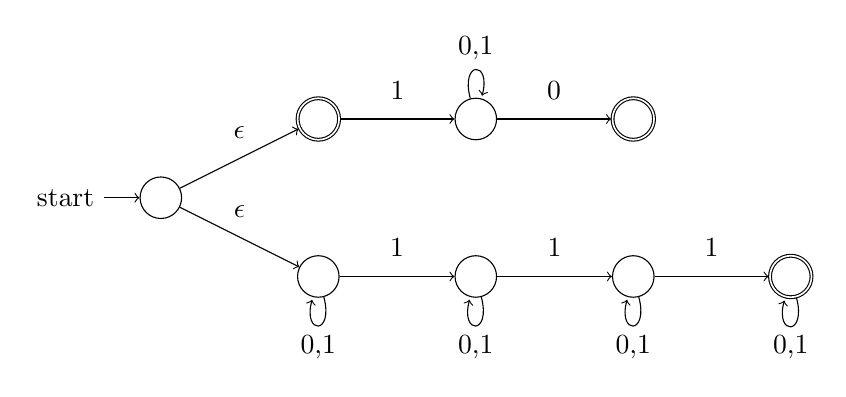
\begin{tikzpicture}

\tikzset{vertex/.style = {shape=circle,draw,minimum size=1.5em}}
\tikzset{edge/.style = {->,> = latex'}}
%verticies
\node[vertex, initial] (1) at  (0,-1) {};
\node[vertex, accepting] (2) at  (2,0) {};
\node[vertex] (3) at  (4,0) {};
\node[vertex, accepting] (4) at  (6,0) {};
\node[vertex] (5) at  (2,-2) {};
\node[vertex] (6) at  (4,-2) {};
\node[vertex] (7) at  (6,-2) {};
\node[vertex, accepting] (8) at  (8,-2) {};
\draw [->] (1) -- (2) node [midway, label=above: {$\epsilon$}] {};
\draw [->] (1) -- (5) node [midway, label=above: {$\epsilon$}] {};
\draw [->] (2) -- (3) node [midway, label=above: {1}] {};
\draw [->] (3) -- (4) node [midway, label=above: {0}] {};
\draw [->] (5) -- (6) node [midway, label=above: {1}] {};
\draw [->] (6) -- (7) node [midway, label=above: {1}] {};
\draw [->] (7) -- (8) node [midway, label=above: {1}] {};
%\path [->] (3) edge[bend left] node [label=below: {0}] {} (2);
%\path [->] (2) edge[bend right=-20] node [label=above: {0}] {} (3);
\path (3) edge[loop above] node {0,1} (3);
\path (5) edge[loop below] node {0,1} (5);
\path (6) edge[loop below] node {0,1} (6);
\path (7) edge[loop below] node {0,1} (7);
\path (8) edge[loop below] node {0,1} (8);

\end{tikzpicture}

\noindent1.8b) \\
\begin{tikzpicture}

\tikzset{vertex/.style = {shape=circle,draw,minimum size=1.5em}}
\tikzset{edge/.style = {->,> = latex'}}
%verticies
\node[vertex, initial] (1) at  (0,-1) {};
\node[vertex] (2) at  (2,0) {};
\node[vertex] (3) at  (4,0) {};
\node[vertex] (4) at  (6,0) {};
\node[vertex] (5) at  (8,0) {};
\node[vertex, accepting] (6) at  (10,0) {};
\node[vertex, accepting] (7) at  (2,-2) {};
\node[vertex, accepting] (8) at  (4,-2) {};
\node[vertex, accepting] (9) at  (2,-4) {};
\draw [->] (1) -- (2) node [midway, label=above: {$\epsilon$}] {};
\draw [->] (1) -- (7) node [midway, label=above: {$\epsilon$}] {};
\draw [->] (2) -- (3) node [midway, label=above: {0}] {};
\draw [->] (3) -- (4) node [midway, label=above: {1}] {};
\draw [->] (4) -- (5) node [midway, label=above: {0}] {};
\draw [->] (5) -- (6) node [midway, label=above: {1}] {};
\draw [->] (7) -- (9) node [midway, label=left: {1}] {};
\path [->] (8) edge[bend left] node [label=below: {0}] {} (7);
\path [->] (7) edge[bend right=-20] node [label=above: {1}] {} (8);
\path (2) edge[loop above] node {0,1} (2);
\path (6) edge[loop above] node {0,1} (6);
\path (7) edge[loop above] node {0} (7);
\path (8) edge[loop above] node {0} (8);
\path (9) edge[loop below] node {1} (9);

\end{tikzpicture}

\noindent1.9a) \\
\begin{tikzpicture}

\tikzset{vertex/.style = {shape=circle,draw,minimum size=1.5em}}
\tikzset{edge/.style = {->,> = latex'}}
%verticies
\node[vertex, initial] (1) at  (0,0) {};
\node[vertex] (2) at  (2,0) {};
\node[vertex] (3) at  (4,0) {};
\node[vertex] (4) at  (6,0) {};
\node[vertex] (5) at  (8,0) {};
\node[vertex] (6) at  (10,0) {};
\node[vertex, accepting] (7) at (5,-2) {};
\node[vertex, accepting] (8) at (5,-4) {};
\draw [->] (1) -- (2) node [midway, label=above: {0,1}] {};
\draw [->] (2) -- (3) node [midway, label=above: {0,1}] {};
\draw [->] (3) -- (4) node [midway, label=above: {0,1}] {};
\draw [->] (4) -- (5) node [midway, label=above: {0,1}] {};
\draw [->] (5) -- (6) node [midway, label=above: {0,1}] {};
\draw [->] (1) -- (7) node [midway, label=left: {$\epsilon$}] {};
\draw [->] (2) -- (7) node [midway, label=left: {$\epsilon$}] {};
\draw [->] (3) -- (7) node [midway, label=left: {$\epsilon$}] {};
\draw [->] (4) -- (7) node [midway, label=left: {$\epsilon$}] {};
\draw [->] (5) -- (7) node [midway, label=left: {$\epsilon$}] {};
\draw [->] (6) -- (7) node [midway, label=left: {$\epsilon$}] {};
\draw [->] (7) -- (8) node [midway, label=right: {1}] {};
\path [->] (8) edge[bend left] node [label=left: {0,1}] {} (7);
%\path [->] (7) edge[bend right=-20] node [label=above: {1}] {} (8);
%\path (2) edge[loop above] node {0,1} (2

\end{tikzpicture}

\noindent1.9b) \\
\begin{tikzpicture}

\tikzset{vertex/.style = {shape=circle,draw,minimum size=1.5em}}
\tikzset{edge/.style = {->,> = latex'}}
%verticies
\node[vertex, initial] (1) at  (0,0) {};

\end{tikzpicture}

\noindent1.10a) \\
\begin{tikzpicture}

\tikzset{vertex/.style = {shape=circle,draw,minimum size=1.5em}}
\tikzset{edge/.style = {->,> = latex'}}
%verticies
\node[vertex, initial, accepting] (1) at  (0,0) {};
\node[vertex] (2) at  (2,0) {};
\node[vertex] (3) at  (4,0) {};
\node[vertex] (4) at  (6,0) {};
\node[vertex, accepting] (5) at  (8,0) {};
\draw [->] (1) -- (2) node [midway, label=below: {$\epsilon$}] {};
\draw [->] (2) -- (3) node [midway, label=below: {1}] {};
\draw [->] (3) -- (4) node [midway, label=below: {1}] {};
\draw [->] (4) -- (5) node [midway, label=below: {1}] {};
\path [->] (5) edge[bend left] node [label=below: {$\epsilon$}] {} (2);
%\path [->] (7) edge[bend right=-20] node [label=above: {1}] {} (8);
\path (5) edge[loop above] node {0,1} (5);
\path (2) edge[loop above] node {0,1} (2);
\path (3) edge[loop above] node {0,1} (3);
\path (4) edge[loop above] node {0,1} (4);

\end{tikzpicture}

\noindent1.10b) \\
\begin{tikzpicture}

\tikzset{vertex/.style = {shape=circle,draw,minimum size=1.5em}}
\tikzset{edge/.style = {->,> = latex'}}
%verticies
\node[vertex, initial, accepting] (0) at  (-1,-1) {};
\node[vertex] (1) at  (0,-1) {};
\node[vertex] (2) at  (2,0) {};
\node[vertex, accepting] (3) at  (6,0) {};
\node[vertex] (4) at  (5,-1) {};
\node[vertex] (5) at  (2,-2) {};
\node[vertex] (6) at  (5,-3) {};
\node[vertex, accepting] (7) at  (6,-2) {};
%edges
\draw [->] (0) -- (1) node [midway, label=above: {$\epsilon$}] {};
\draw [->] (1) -- (2) node [midway, label=above: {0}] {};
\draw [->] (1) -- (5) node [midway, label=above: {1}] {};
\draw [->] (2) -- (3) node [midway, label=above: {0}] {};
\draw [->] (2) -- (4) node [midway, label=above: {1}] {};
\draw [->] (3) -- (7) node [midway, label=right: {1}] {};
\draw [->] (5) -- (4) node [midway, label=right: {0}] {};
\draw [->] (4) -- (7) node [midway, label=right: {0}, pos=0.2] {};
\draw [->] (4) -- (6) node [midway, label=right: {1}] {};
\draw [->] (5) -- (6) node [midway, label=right: {1}] {};
\draw [->] (7) -- (6) node [midway, label=right: {1}] {};
\path [->] (3) edge[bend left=-50] node [label=above: {$\epsilon$}] {} (1);
\path [->] (7) edge[bend left=100] node [label=below: {$\epsilon$}] {} (1);
\path (3) edge[loop above] node {0} (3);
\path (7) edge[loop right] node {0} (7);

\end{tikzpicture}

\noindent1.10c) \\
\begin{tikzpicture}

\tikzset{vertex/.style = {shape=circle,draw,minimum size=1.5em}}
\tikzset{edge/.style = {->,> = latex'}}
%verticies
\node[vertex, initial, accepting] (0) at  (0,0) {};
\node[vertex] (1) at  (2,0) {};
%edges
\draw [->] (0) -- (1) node [midway, label=above: {$\epsilon$}] {};

\end{tikzpicture}

\noindent1.12) \\
\begin{tikzpicture}

\tikzset{vertex/.style = {shape=circle,draw,minimum size=1.5em}}
\tikzset{edge/.style = {->,> = latex'}}
%verticies
\node[vertex, initial] (1) at  (0,0) {};
\node[vertex, accepting] (2) at  (2,0) {};
\node[vertex] (3) at  (4,0) {};
\node[vertex, accepting] (4) at  (6,0) {};
\node[vertex] (5) at  (3,-3) {};
%edges
\draw [->] (1) -- (5) node [midway, label=above: {a}] {};
\draw [->] (2) -- (3) node [midway, label=above: {a}] {};
\draw [->] (3) -- (5) node [midway, label=above: {b}] {};
\draw [->] (4) -- (5) node [midway, label=above: {b}] {};
\path [->] (1) edge[bend right=-20] node [label=above: {b}] {} (2);
\path [->] (2) edge[bend left] node [label=below: {b}] {} (1);
\path [->] (3) edge[bend right=-20] node [label=above: {a}] {} (4);
\path [->] (4) edge[bend left] node [label=above: {a}] {} (3);
\path (5) edge[loop below] node {a,b} (5);

\end{tikzpicture}

\noindent R = b(bb)*(aa)* \\

\noindent1.13) \\
\begin{tikzpicture}

\tikzset{vertex/.style = {shape=circle,draw,minimum size=1.5em}}
\tikzset{edge/.style = {->,> = latex'}}
%verticies
\node[vertex, initial, accepting] (1) at  (0,0) {q0};
\node[vertex] (2) at  (2,0) {q0,1};
\node[vertex, accepting] (3) at  (4,0) {q0,1,2};
\node[vertex] (4) at  (2,-2) {q0,3};
\node[vertex] (5) at  (4,-2) {q0,1,2,3};
%edges
\draw [->] (1) -- (2) node [midway, label=above: {1}] {};
\draw [->] (2) -- (3) node [midway, label=above: {1}] {};
\draw [->] (3) -- (5) node [midway, label=right: {1}] {};
\draw [->] (4) -- (5) node [midway, label=below: {1}] {};
\path [->] (2) edge[bend right=-20] node [label=right: {0}] {} (4);
\path [->] (4) edge[bend left] node [label=left: {0}] {} (2);
\path (1) edge[loop above] node {0} (1);
\path (3) edge[loop above] node {0} (3);
\path (5) edge[loop right] node {0,1} (5);

\end{tikzpicture}

\noindent1.16a) \\
\begin{tikzpicture}

\tikzset{vertex/.style = {shape=circle,draw,minimum size=1.5em}}
\tikzset{edge/.style = {->,> = latex'}}
%verticies
\node[vertex, initial, accepting] (1) at  (0,0) {q1};
\node[vertex] (2) at  (2,0) {q2};
\node[vertex, accepting] (3) at  (0,-2) {q1,2};
\node[vertex] (4) at  (2,-2) {$\emptyset$};
%edges
\draw [->] (1) -- (3) node [midway, label=left: {a}] {};
\draw [->] (2) -- (4) node [midway, label=right: {a}] {};
\path [->] (1) edge[bend right=-20] node [label=above: {b}] {} (2);
\path [->] (2) edge[bend left] node [label=below: {b}] {} (1);
\path (3) edge[loop below] node {a,b} (3);

\end{tikzpicture}

\noindent1.16b) \\
\begin{tikzpicture}

\tikzset{vertex/.style = {shape=circle,draw,minimum size=1.5em}}
\tikzset{edge/.style = {->,> = latex'}}
%verticies
\node[vertex] (1) at  (2,0) {$\emptyset$};
\node[vertex, initial=right, accepting] (2) at  (0,0) {q1,2};
\node[vertex, accepting] (3) at  (0,-2) {q2,3};
\node[vertex, accepting] (4) at  (2,-2) {q1,2,3};
%edges
\draw [->] (2) -- (1) node [midway, label=above: {b}] {};
\draw [->] (2) -- (4) node [midway, label=right: {a}] {};
\draw [->] (4) -- (3) node [midway, label=below: {b}] {};
\draw [->] (3) -- (2) node [midway, label=right: {a}] {};
%\path [->] (1) edge[bend right=-20] node [label=above: {b}] {} (2);
%\path [->] (2) edge[bend left] node [label=below: {b}] {} (1);
\path (1) edge[loop above] node {a,b} (1);
\path (3) edge[loop below] node {b} (3);
\path (4) edge[loop below] node {a} (4);

\end{tikzpicture}

\noindent1.17a) \\
\begin{tikzpicture}

\tikzset{vertex/.style = {shape=circle,draw,minimum size=1.5em}}
\tikzset{edge/.style = {->,> = latex'}}
%verticies
\node[vertex, initial, accepting] (1) at  (0,-1) {1};
\node[vertex] (2) at  (2,-1) {2};
\node[vertex] (3) at  (4,0) {3};
\node[vertex] (4) at  (6,0) {4};
\node[vertex] (5) at  (4,-2) {5};
\node[vertex] (6) at  (6,-2) {6};
%edges
\draw [->] (1) -- (2) node [midway, label=above: {0}] {};
\draw [->] (2) -- (3) node [midway, label=right: {0}] {};
\draw [->] (3) -- (4) node [midway, label=below: {1}] {};
\draw [->] (2) -- (5) node [midway, label=right: {1}] {};
\draw [->] (5) -- (6) node [midway, label=above: {0}] {};
\path [->] (5) edge[bend left] node [label=below: {$\epsilon$}] {} (1);
\path [->] (6) edge[bend left] node [label=below: {$\epsilon$}] {} (1);
\path [->] (4) edge[bend left=-40] node [label=above: {$\epsilon$}] {} (1);
%\path (1) edge[loop above] node {a,b} (1);
%\path (3) edge[loop below] node {b} (3);
%\path (4) edge[loop below] node {a} (4);

\end{tikzpicture}

\noindent 1.18) \\
a) $1\Sigma^\ast0$ \\
b) $\Sigma^\ast1\Sigma^\ast1\Sigma^\ast1\Sigma^\ast$ \\
c) $\Sigma^\ast0101\Sigma^\ast$ \\
d) $\Sigma\Sigma0\Sigma^\ast$ \\
e) $(0\cup1\Sigma)(\Sigma\Sigma)^\ast$ \\
f) $0^\ast(10^+)^\ast1^\ast$ \\
g) $(\in\cup\Sigma)^5$ \\
h) $\in\cup\Sigma\cup0\Sigma\cup10\cup0\Sigma\Sigma\cup10\Sigma\cup110\Sigma^3\Sigma^+$ \\
i) $(1\Sigma)^*(\in\cup1)$ \\
j) $00^+\cup100^+\cup0^+\cup0^+10^+\cup00^+1$ \\
k) $0\cup\in$ \\
l) $1^*(01^*01^*)\cup0^*10^*10^*$ \\
m) $\emptyset$ \\
n) $\Sigma^+$ \\

\noindent 1.20) \\
a) Members: ab, abb \\
   Non-Members: ba, bba \\ \\
b) Members: abab, ababab \\
Non-Members: aba, bab \\ \\
c) Members: aaaaa, bbb \\
Non-Members: baab, bbaa \\ \\
d) Members: aaa, aaaaaaaaa \\
Non-Members: a, aa \\ \\
e) Members: aba, aabbaa \\
Non-Members: ab, a \\ \\
f) Members: aba, bab \\
Non-Members: ab, ba \\ \\
g) Members: ab, b \\
Non-Members: ba, b \\ \\
h) Members: a, ba \\
Non-Members: b, ab \\

\noindent1.21) \\
\begin{tikzpicture}

\tikzset{vertex/.style = {shape=circle,draw,minimum size=1.5em}}
\tikzset{edge/.style = {->,> = latex'}}
%verticies
\node[vertex, initial] (1) at  (0,0) {1};
\node[vertex, accepting] (2) at  (2,0) {2};
%edges
%\draw [->] (1) -- (2) node [midway, label=above: {0}] {};
\path [->] (1) edge[bend right=-20] node [label=above: {b}] {} (2);
\path [->] (2) edge[bend left] node [label=below: {b}] {} (1);
\path (1) edge[loop above] node {a} (1);
\path (2) edge[loop above] node {a} (2);
%\path (4) edge[loop below] node {a} (4);

\end{tikzpicture}

\noindent Step 1: \\
\begin{tikzpicture}

\tikzset{vertex/.style = {shape=circle,draw,minimum size=1.5em}}
\tikzset{edge/.style = {->,> = latex'}}
%verticies
\node[vertex, initial] (0) at  (0,0) {S};
\node[vertex] (1) at  (2,0) {1};
\node[vertex] (2) at  (4,0) {2};
\node[vertex, accepting] (3) at  (6,0) {F};
%edges
\draw [->] (0) -- (1) node [midway, label=above: {$\epsilon$}] {};
\path [->] (1) edge[bend right=-20] node [label=above: {b}] {} (2);
\path [->] (2) edge[bend left] node [label=below: {b}] {} (1);
\draw [->] (2) -- (3) node [midway, label=above: {$\epsilon$}] {};
\path (1) edge[loop above] node {a} (1);
\path (2) edge[loop above] node {a} (2);
%\path (4) edge[loop below] node {a} (4);

\end{tikzpicture}

\noindent Step 2: \\
\begin{tikzpicture}

\tikzset{vertex/.style = {shape=circle,draw,minimum size=1.5em}}
\tikzset{edge/.style = {->,> = latex'}}
%verticies
\node[vertex, initial] (0) at  (0,0) {S};
\node[vertex] (1) at  (2,0) {2};
\node[vertex, accepting] (2) at  (4,0) {F};
%edges
\draw [->] (0) -- (1) node [midway, label=above: {a$^\ast$b}] {};
\draw [->] (1) -- (2) node [midway, label=above: {$\epsilon$}] {};
\path (1) edge[loop above] node {a} (1);
\path (1) edge[loop below] node {ba$^\ast$b} (1);
%\path (4) edge[loop below] node {a} (4);

\end{tikzpicture}

\noindent Step 3: \\
\begin{tikzpicture}

\tikzset{vertex/.style = {shape=circle,draw,minimum size=1.5em}}
\tikzset{edge/.style = {->,> = latex'}}
%verticies
\node[vertex, initial] (0) at  (0,0) {S};
\node[vertex] (1) at  (2,0) {2};
\node[vertex, accepting] (2) at  (4,0) {F};
%edges
\draw [->] (0) -- (1) node [midway, label=above: {a$^\ast$b}] {};
\draw [->] (1) -- (2) node [midway, label=above: {$\epsilon$}] {};
\path (1) edge[loop above] node {a$\cup$ba$^\ast$b} (1);
%\path (4) edge[loop below] node {a} (4);

\end{tikzpicture}

\noindent Step 4: \\
\begin{tikzpicture}

\tikzset{vertex/.style = {shape=circle,draw,minimum size=1.5em}}
\tikzset{edge/.style = {->,> = latex'}}
%verticies
\node[vertex, initial] (0) at  (0,0) {S};
\node[vertex, accepting] (1) at  (4,0) {F};
%edges
\draw [->] (0) -- (1) node [midway, label=above: {a$^\ast$b(a$\cup$ba$^\ast$b)}] {};
%\path (4) edge[loop below] node {a} (4);

\end{tikzpicture}
Regular Expression: a$^\ast$b(a$\cup$ba$^\ast$b) \\

\noindent1.21b) \\
\begin{tikzpicture}

\tikzset{vertex/.style = {shape=circle,draw,minimum size=1.5em}}
\tikzset{edge/.style = {->,> = latex'}}
%verticies
\node[vertex, initial, accepting] (1) at  (0,0) {1};
\node[vertex] (2) at  (2,0) {2};
\node[vertex, accepting] (3) at  (1,-2) {3};
%edges
\draw [->] (1) -- (2) node [midway, label=above: {a,b}] {};
\draw [->] (3) -- (1) node [midway, label=left: {a}] {};
\path [->] (2) edge[bend right=-20] node [label=right: {b}] {} (3);
\path [->] (3) edge[bend left] node [label=left: {b}] {} (2);
\path (2) edge[loop above] node {a} (2);
%\path (3) edge[loop below] node {b} (3);
%\path (4) edge[loop below] node {a} (4);

\end{tikzpicture}

\noindent Step 1: \\
\begin{tikzpicture}

\tikzset{vertex/.style = {shape=circle,draw,minimum size=1.5em}}
\tikzset{edge/.style = {->,> = latex'}}
%verticies
\node[vertex, initial] (0) at  (0,0) {S};
\node[vertex] (1) at  (2,0) {1};
\node[vertex] (2) at  (4,0) {2};
\node[vertex] (3) at  (3,-2) {3};
\node[vertex, accepting] (4) at  (1,-2) {F};
%edges
\draw [->] (0) -- (1) node [midway, label=above: {$\epsilon$}] {};
\draw [->] (1) -- (4) node [midway, label=left: {$\epsilon$}] {};
\draw [->] (3) -- (4) node [midway, label=below: {$\epsilon$}] {};
\draw [->] (1) -- (2) node [midway, label=above: {a,b}] {};
\draw [->] (3) -- (1) node [midway, label=left: {a}] {};
\path [->] (2) edge[bend right=-20] node [label=right: {b}] {} (3);
\path [->] (3) edge[bend left] node [label=right: {b}, pos=0.2] {} (2);
\path (2) edge[loop above] node {a} (2);
%\path (3) edge[loop below] node {b} (3);
%\path (4) edge[loop below] node {a} (4);

\end{tikzpicture}

\noindent Step 2: \\
\begin{tikzpicture}

\tikzset{vertex/.style = {shape=circle,draw,minimum size=1.5em}}
\tikzset{edge/.style = {->,> = latex'}}
%verticies
\node[vertex, initial] (0) at  (0,0) {S};
\node[vertex] (1) at  (2,0) {1};
\node[vertex] (2) at  (4,0) {2};
\node[vertex] (3) at  (3,-2) {3};
\node[vertex, accepting] (4) at  (1,-2) {F};
%edges
\draw [->] (0) -- (1) node [midway, label=above: {$\epsilon$}] {};
\draw [->] (1) -- (4) node [midway, label=left: {$\epsilon$}] {};
\draw [->] (3) -- (4) node [midway, label=below: {$\epsilon$}] {};
\draw [->] (1) -- (2) node [midway, label=above: {a$\cup$b}] {};
\draw [->] (3) -- (1) node [midway, label=left: {a}] {};
\path [->] (2) edge[bend right=-20] node [label=right: {b}] {} (3);
\path [->] (3) edge[bend left] node [label=right: {b}, pos=0.2] {} (2);
\path (2) edge[loop above] node {a} (2);

\end{tikzpicture}

\noindent Step 3: \\
\begin{tikzpicture}

\tikzset{vertex/.style = {shape=circle,draw,minimum size=1.5em}}
\tikzset{edge/.style = {->,> = latex'}}
%verticies
\node[vertex, initial] (0) at  (0,0) {S};
\node[vertex] (2) at  (4,0) {2};
\node[vertex] (3) at  (3,-2) {3};
\node[vertex, accepting] (4) at  (1,-2) {F};
%edges
\draw [->] (0) -- (2) node [midway, label=above: {a$\cup$b}] {};
\draw [->] (0) -- (4) node [midway, label=left: {$\epsilon$}] {};
\path [->] (2) edge[bend left] node [label=right: {b}] {} (3);
\path [->] (3) edge[bend right=-20] node [label=right: {b}, pos=0.2] {} (2);
\path [->] (3) edge[bend right=-60] node [label=left: {a(a$\cup$b)}] {} (2);
\path [->] (3) edge[bend left=-20] node [label=above: {a}] {} (4);
\path [->] (3) edge[bend left] node [label=below: {$\epsilon$}] {} (4);
\path (2) edge[loop above] node {a} (2);

\end{tikzpicture}

\noindent Step 4: \\
\begin{tikzpicture}

\tikzset{vertex/.style = {shape=circle,draw,minimum size=1.5em}}
\tikzset{edge/.style = {->,> = latex'}}
%verticies
\node[vertex, initial] (0) at  (0,0) {S};
\node[vertex] (2) at  (4,0) {2};
\node[vertex] (3) at  (3,-2) {3};
\node[vertex, accepting] (4) at  (1,-2) {F};
%edges
\draw [->] (0) -- (2) node [midway, label=above: {a$\cup$b}] {};
\draw [->] (0) -- (4) node [midway, label=left: {$\epsilon$}] {};
\draw [->] (3) -- (4) node [midway, label=below: {$\epsilon\cup$a}] {};
\path [->] (2) edge[bend left] node [label=right: {b}] {} (3);
\path [->] (3) edge[bend right=-20] node [label=left: {a(a$\cup$b)$\cup$b}] {} (2);
\path (2) edge[loop above] node {a} (2);

\end{tikzpicture}

\noindent Step 5: \\
\begin{tikzpicture}

\tikzset{vertex/.style = {shape=circle,draw,minimum size=1.5em}}
\tikzset{edge/.style = {->,> = latex'}}
%verticies
\node[vertex, initial] (0) at  (0,0) {S};
\node[vertex] (3) at  (3,-2) {3};
\node[vertex, accepting] (4) at  (1,-2) {F};
%edges
\draw [->] (0) -- (4) node [midway, label=left: {$\epsilon$}] {};
\draw [->] (3) -- (4) node [midway, label=below: {$\epsilon\cup$a}] {};
\draw [->] (0) -- (3) node [midway, label=right: {(a$\cup$b)a$^*$b}] {};
\path (3) edge[loop right] node {(a(a$\cup$b)$\cup$b)a$^*$b} (3);

\end{tikzpicture}

\noindent Step 6: \\
\begin{tikzpicture}

\tikzset{vertex/.style = {shape=circle,draw,minimum size=1.5em}}
\tikzset{edge/.style = {->,> = latex'}}
%verticies
\node[vertex, initial] (0) at  (0,0) {S};
\node[vertex, accepting] (4) at  (1,-2) {F};
%edges
\path [->] (0) edge[bend right=-20] node [label=right: {((a$\cup$b)a$^*$b(a(a$\cup$b)$\cup$b)a$^*$b)$^*$($\epsilon\cup$a)}] {} (4);
\path [->] (0) edge[bend right] node [label=left: {$\epsilon$}] {} (4);

\end{tikzpicture}

\noindent Step 7: \\
\begin{tikzpicture}

\tikzset{vertex/.style = {shape=circle,draw,minimum size=1.5em}}
\tikzset{edge/.style = {->,> = latex'}}
%verticies
\node[vertex, initial] (0) at  (0,0) {S};
\node[vertex, accepting] (4) at  (1,-2) {F};
%edges
\draw [->] (0) -- (4) node [midway, label=right: {$\epsilon\cup$((a$\cup$b)a$^*$b(a(a$\cup$b)$\cup$b)a$^*$b)$^*$($\epsilon\cup$a)}] {};

\end{tikzpicture}

Regular Expression = $\epsilon\cup$((a$\cup$b)a$^*$b(a(a$\cup$b)$\cup$b)a$^*$b)$^*$($\epsilon\cup$a)

\noindent 1.22a): \\
\begin{tikzpicture}

\tikzset{vertex/.style = {shape=circle,draw,minimum size=1.5em}}
\tikzset{edge/.style = {->,> = latex'}}
%verticies
\node[vertex, initial] (1) at  (0,0) {};
\node[vertex] (2) at  (2,0) {};
\node[vertex] (3) at  (4,0) {};
\node[vertex] (4) at  (6,0) {};
\node[vertex, accepting] (5) at  (8,0) {};
\node[vertex] (6) at  (4,-3) {};
%edges
\draw [->] (1) -- (2) node [midway, label=above: {/}] {};
\draw [->] (2) -- (3) node [midway, label=above: {\#}] {};
\draw [->] (3) -- (4) node [midway, label=above: {\#}] {};
\draw [->] (4) -- (5) node [midway, label=above: {/}] {};
\draw [->] (1) -- (6) node [midway, label=left: {a,b,\#}, pos=0.2] {};
\draw [->] (2) -- (6) node [midway, label=left: {a,b,/}, pos=0.2] {};
\draw [->] (3) -- (6) node [midway, label=right: {/}, pos=0.2] {};
\draw [->] (4) -- (6) node [midway, label=right: {a,b,\#}, pos=0.2] {};
\draw [->] (5) -- (6) node [midway, label=right: {a,b,\#,/}, pos=0.2] {};
\path (3) edge[loop above] node {a,b} (3);
\path (6) edge[loop below] node {a,b,\#,/} (6);

\end{tikzpicture}

\noindent 1.22b) Regular Expression = /\#(a$\cup$b)$^*$\#/ \\


\end{document}